\section{Concept}\label{6sec:concept}

The communication with the central server was required to be via the 
MQTT protocol for every part of the Smart City Project.
It is designed to still function even with high latency's 
and limited bandwidth, 
so its something that could also realistically be used 
in a real world implementation of a Smart City.

\noindent
As mentioned in Section \ref{6sec:intro},
CARLA was also already decided as the way to simulate the cars. 
The rest of the development of the concept was mostly driven by small experiments 
with the example scripts from the CARLA Python API. 
These covered spawning NPCs, Non-Player-Characters, 
which autonomously drive around the city,
or changing the weather in the simulation.

\noindent
The example scripts also contain a basic manually drivable car.
This car object already has multiple sensors implemented for it,
including a collision sensor.
This would provide a easy way to fulfill the crash detection part of the task
and it was then possible to write the formal requirements for the system.

\vspace{-18pt}
\subsection{Requirements}
The Requirements, as depicted in Figure \ref{6fig:reqTable}, 
were published to the Wiki of the GitHub repository on May 5th.

\noindent
In the conclusion these will be looked at again, 
to see if all requirements are satisfied by the implementation

\vspace{-4pt}
\begin{figure}[H]
  \centering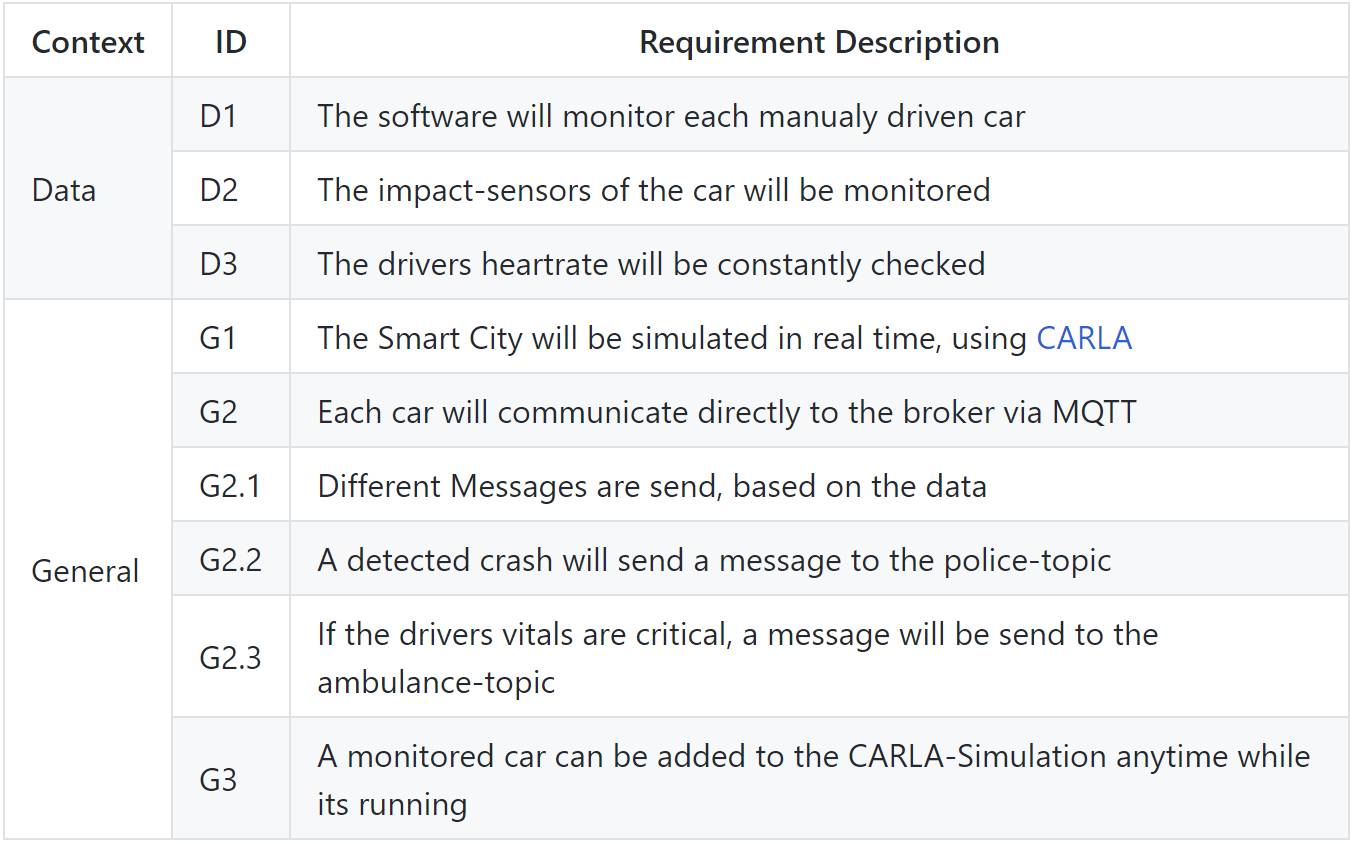
\includegraphics[width=1.0\linewidth]{chapters/chapter6_bruno/Figures/requirements.png}
  \caption{Table of requirements on GitHub}
  \label{6fig:reqTable}
\end{figure}
\vspace{-34pt}
\subsection{Sequence Chart}

\noindent
As the final part of the concept, the UML Sequence Chart seen in 
Figure \ref{6fig:sequenceChart1} was created. 
Although the exact message arguments are slightly altered in the final implementation,
The sequence of events is still the same.
Only the \emph{Driver} and the \emph{Auto} lifelines 
are actually part of this section of the project, 
but the rest also appear here,
to show how the whole Smart City works in these situations. 
\\
\newline
The first loop in Figure \ref{6fig:sequenceChart1} represents the vitals monitor 
that runs in parallel to the crash detection.
It request the heart rate from the sensor
and checks if it is outside the normal range.
If the value is dangerous, a message to the server is send,
containing information about the driver, the position of the car
and the heart rate.
The server then processes this information and sends a message to the ambulances,
but this is again, not part of this section of the project Smart City.

\begin{figure}[H]
  \centering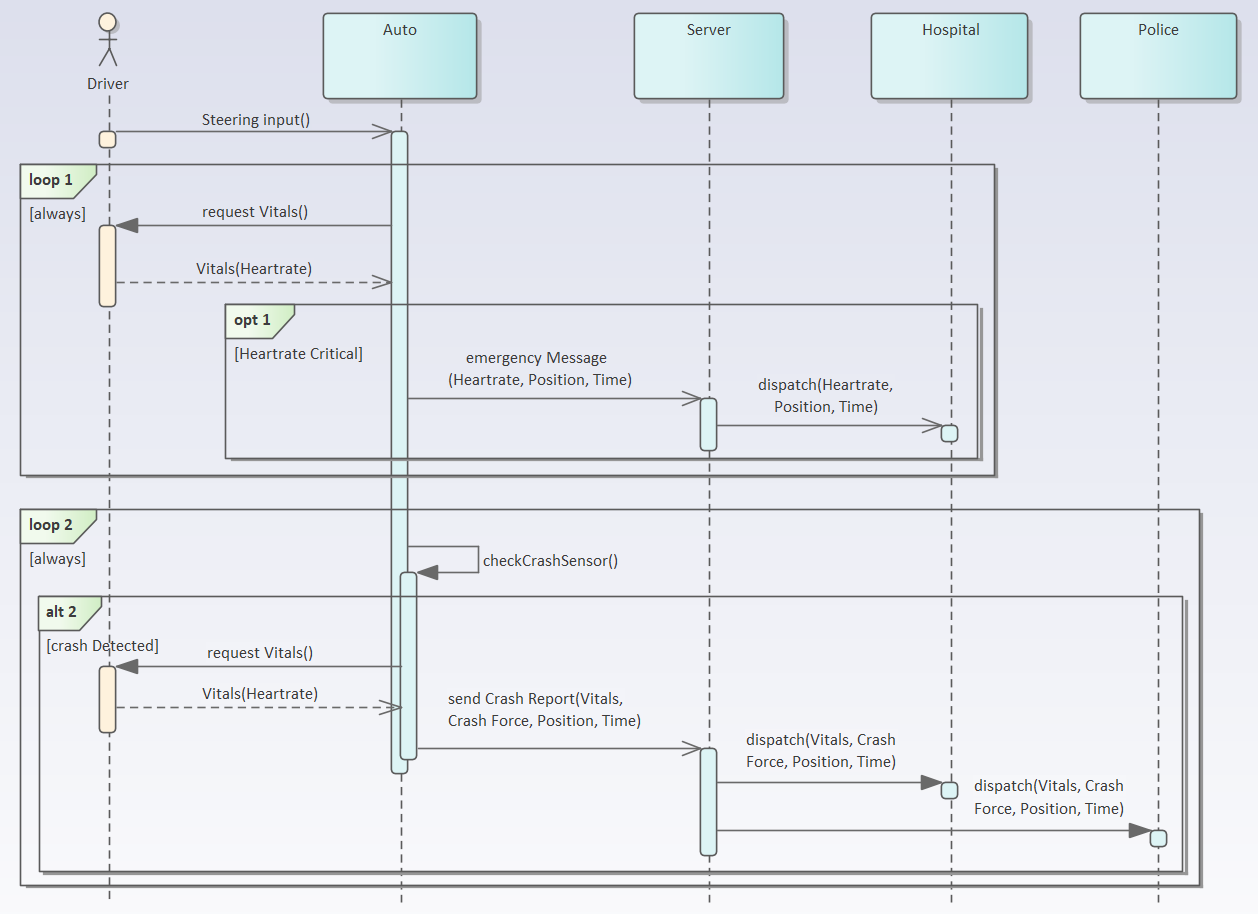
\includegraphics[width=1.0\linewidth]{chapters/chapter6_bruno/Figures/sequence1.png}
  \caption{Sequence Charts}
  \label{6fig:sequenceChart1}
\end{figure}

\noindent
The second loop shows how the crash detection works
in a very similar way.
The crash sensor is constantly monitored while the car is running.
If a collision is detected, the system gets the heart rate of the driver
and sends the message that a crash has occurred.
This message includes all known information about the crash.
If the heart rate is also critical,
a second message is send, like the one in the first loop.